\selectlanguage{english}
\chapter[Improving Model Transfer]{Improving Model Transfer}
\label{ch:model-transfer}

In this chapter we will focus on zero-shot model transfer. In Chapter \ref{ch:model-vs-data} we demonstrated that model transfer could be an effective and efficient approach for cross-lingual transfer when using a high-capacity model on the target language. Therefore, for this approach to be effective, it is crucial to use the most powerful models available. Currently, these models are the text-to-text Large Language Models (LLMs). However, using LLMs for zero-shot cross-lingual sequence labeling is not straightforward. In this chapter we will introduce a constrained decoding algorithm that effectively addresses this issue. A comprehensive empirical evaluation across multiple tasks and languages demonstrates that, when our method is applied to an LLM, it helps not only to improve over the unconstrained beam search baseline but also to outperform the zero-shot cross-lingual capabilities of encoder-only models, especially for languages that significantly differ from English.

\section{Motivation and contributions}
\label{sc6:intro}

In Chapter \ref{ch:model-vs-data}, we demonstrated that the performance of zero-shot cross-lingual transfer can be significantly enhanced by using a high-capacity model for the target language. However, we only employed encoder-only models such as XLM-RoBERTa-large (\cite{conneau-etal-2020-unsupervised}), which has 561 million parameters and was trained on approximately 295 billion tokens. However, as mentioned in Chapter \ref{sc:deep-learning-sota}, the most powerful models currently available are text-to-text Large Language Models (LLMs) like T5 (\cite{DBLP:journals/jmlr/RaffelSRLNMZLL20-T5}), LLaMA (\cite{llama3modelcard}), and GPT-4 (\cite{openai2024gpt4technicalreport}). These models have demonstrated superior capabilities in a wide range of NLP tasks, including the ability to solve tasks for which they were not explicitly trained. Consequently, efforts to scale NLP models have primarily focused on text generation models. As shown in Table \ref{tab:model-size}, the latest generation of LLMs have significantly more parameters and were trained on much larger datasets compared to XLM-RoBERTa.


\begin{table}[!thp]
% \vspace{-1em}
\caption{\label{tab:model_size}
Performance comparison of \jola{} across different model sizes: Llama-3.2-1B-Instruct, Llama-3.2-3B-Instruct, and Llama-3.1-70B-Instruct.
}
\resizebox{\columnwidth}{!}{
\begin{tabular}{l|l|cccccc}
\toprule
                     &            & \multicolumn{2}{c}{\textbf{Reasoning}} & \multicolumn{2}{c}{\textbf{Understanding}}  & \multicolumn{2}{c}{\textbf{Generation}}  \\
\cmidrule(lr){3-4}\cmidrule(lr){5-6}\cmidrule(lr){7-8}
                     &            & SIQA      & WinoGrande & Law           & Physics & E2E\_NLG   & WEG\_NLG \\
\midrule
\multirow{3}{*}{1B}  & \textbf{zero\_shot} & 23.34     & 2.45       & 9.00          & 3.00    & 7.59       & 6.32     \\
                     & \textbf{LoRA}       & 31.92     & 29.13      & 12.00         & 12.00   & 16.95      & 16.52    \\
                     & \textbf{our}        & 37.82     & 49.33      & 16.00         & 19.00   & 26.89      & 27.72    \\
\midrule
\multirow{3}{*}{3B}  & \textbf{zero\_shot} & 27.33     & 5.05       & 14.00         & 8.00    & 7.48       & 22.42    \\
                     & \textbf{LoRA}       & 50.09     & 43.28      & 15.00         & 21.00   & 23.76      & 28.19    \\
                     & \textbf{our}        & 63.05     & 56.67      & 20.00         & 32.00   & 34.78      & 31.47    \\
\midrule
\multirow{3}{*}{70B} & \textbf{zero\_shot} & 51.28     & 29.83      & 37.00         & 32.00   & 10.26      & 24.15    \\
                     & \textbf{LoRA}       & 61.78     & 56.54      & 42.00         & 38.00   & 35.87      & 42.81    \\
                     & \textbf{our}        & 72.17     & 70.26      & 51.00         & 45.00   & 46.18      & 57.12    \\
\bottomrule
\end{tabular}
}
% \vspace{-1.2em}
\end{table}

LLM models have already been proven effective for Information Extraction and sequence labeling tasks in monolingual evaluations in English (\cite{DBLP:journals/corr/abs-2305-15444, sainz2024gollie}). However, their performance still lags behind encoder-only models in multilingual sequence labeling (\cite{DBLP:conf/semeval/FetahuKCRM23}). For low-resource languages, such as African languages, \cite{DBLP:conf/africanlp/OjoO23} demonstrated that most text-to-text LLMs for named entity recognition do not perform well at all when evaluated in a zero-shot setting. Their results are reproduced in Table \ref{tab6:howgoodafrican}. The table shows that the performance of LLMs is significantly lower than that of XLM-RoBERTa-large. This is a surprising result, given that many of the LLMs have been trained on much larger multilingual datasets and have significantly more parameters than XLM-RoBERTa-large. Thus, the question arises: why do LLMs perform poorly in zero-shot cross-lingual sequence labeling tasks?

\definecolor{Color}{gray}{0.9}
\begin{table}[htb]
    \begin{center}
    \resizebox{\textwidth}{!}{
    \begin{tabular}{llrrrrrrrrrrrrrrrrrrrr}
    \toprule
    \textbf{Model} &\textbf{Size} &\textbf{amh} &\textbf{bam}  &\textbf{bbj} &\textbf{ewe} &\textbf{hau} &\textbf{ibo} &\textbf{kin} &\textbf{lug} &\textbf{luo} &\textbf{mos} &\textbf{nya} &\textbf{pcm} &\textbf{sna} &\textbf{swa} &\textbf{tsn} &\textbf{twi} &\textbf{wol} &\textbf{xho} &\textbf{yor} &\textbf{zul} \\
    \midrule
    \multicolumn{2}{l}{\texttt{Fine-tune: SotA}} \\
    \rowcolor{Color}
    AfroXLMR-large & 550M & \textbf{78.0}  &\textbf{79.0} &\textbf{90.3} &75.2 &\textbf{85.4} &\textbf{88.9} &\textbf{86.8} &\textbf{88.9} &\textbf{75.3} &\textbf{73.5} &\textbf{92.4} &\textbf{90.0} &\textbf{96.1} &\textbf{92.7} &\textbf{88.9} &\textbf{79.2} &\textbf{83.8} &\textbf{89.2} &\textbf{67.9} &\textbf{90.6} \\
    \midrule
    \multicolumn{2}{l}{\texttt{Prompting of LLMs}} \\
    GPT-4 & - &28.5  &52.7 &50.3 &\textbf{75.6} &64.9 &56.0 &55.1 &73.3 &49.8 &60.2 &63.6 &64.7 &33.4 &71.5 &64.6 &58.6 &67.9 &28.4 &58.3 &34.9 \\
    AYA & - &14.1 &7.1 &20.0 &26.5 &34.5 &28.2 &30.8 &16.3 &12.7 &34.4 &21.7 &27.4 &13.4\definecolor{Color}{gray}{0.9} &35.6 &29.4 &18.9 &14.5 &4.2 &17.5 &11.4  \\
    mT0 & 13B &0.0 &0.0 &0.0 &0.1 &0.0 &0.0 &0.0 &0.0 &0.0 &0.0 &0.0 &0.0 &0.0 &0.0 &0.0 &0.0 &0.0 &0.0 &0.0 &0.0  \\
    mT0-MT & 13B &0.0 &0.0 &0.0 &0.1 &0.0 &0.0 &0.0 &0.0 &0.0 &0.0 &0.0 &0.0 &0.0 &0.0 &0.0 &0.0 &0.0 &0.0 &0.0 &0.0  \\
    LLaMa 2 & 13B &0.0 &13.8 &12.3 &25.1 &22.1 &22.0 &23.1 &27.5 &19.0 &11.0 &20.0 &27.5 &11.3 &25.8 &26.2 &20.7 &16.0 &8.1 &15.1 &9.0  \\
    \bottomrule
    \end{tabular}
    }
    \caption{Comparison of F1-score of various LLMs with that of the current state of the art result in Masakhaner 2.0. Table reproduced from \cite{DBLP:conf/africanlp/OjoO23}.
    }
    \label{tab6:howgoodafrican}
    \end{center}

    \end{table}


In this chapter, we investigate the performance of LLMs in zero-shot cross-lingual sequence labeling tasks. Our contributions are as follows:

\paragraph{We identify the challenges faced by text-to-text models for zero-shot sequence labeling:} In this setting we must first establish a text-based input and output representation for the specific task. However, current text-to-text models are tailored for generating free-form text. As our experiments demonstrate, models fail to strictly adhere to the output structure. Moreover, as demonstrated by our experiments, text-to-text models often produce outputs mixing the source language and the target language, which compromises their performance. These issues are illustrated in Figure \ref{fig6:constrained_unconstrained}, where the incorrect output mixes English and Basque (Turkiako-Turkish) and incorrectly segments the organization entity ``Realean''.

\begin{figure}[htb]
    \centering
    \includegraphics[width=\textwidth]{Capitulos/6_ModelTransfer/diagramas/ConstrainedUnconstrainedDecoding.pdf}
    \caption{Comparison between a valid (top green) and invalid (bottom red) output structure to represent a Named Entity Recognition task. English translation: (They) played in Real and in the Turkish national team.}
    \label{fig6:constrained_unconstrained}
\end{figure}

\paragraph{We propose a constrained decoding algorithm for text-to-text models:} We introduce a constrained decoding algorithm that enforces the output structure of the target task. Our method can be seamlessly integrated with any text-to-text model without any significant increase in the decoding cost. Although constrained generation has been previously explored in a monolingual setting (\cite{liu-etal-2022-autoregressive}), we adapt and extend this approach for zero-shot cross-lingual IE. Our new decoding algorithm is evaluated on three popular IE tasks for 25 languages of varied morphological characteristics. Empirical results indicate that our method, when applied to an LLM such as mT0-XL (\cite{DBLP:conf/acl/MuennighoffWSRB23}), not only surpasses the unconstrained beam search baseline but also outperforms the zero-shot cross-lingual performance of encoder-only models. Our method is especially successful for languages that significantly differ from English.

To the best of our knowledge, our new technique achieves the best zero-shot model-based cross-lingual transfer results to date.


\section{Related Work}
In this section, we focus first on related work concerning large language models (LLMs) for sequence labeling. In the second part of the related work, we review prior research on constrained decoding.

\subsection{LLMs for sequence labeling}

The introduction of models like T5 (\cite{DBLP:journals/jmlr/RaffelSRLNMZLL20-T5}) and GPT (\cite{radford2019language}) revolutionized NLP by adopting a text-to-text approach, enabling models to handle a wide array of tasks with a single training objective. Consequently, all NLP tasks can be framed as text-to-text tasks, where the input is a description of the task or a prompt, and the output is the desired result (\cite{chung-flan-instruction-models}). Scaling these models in both the amount of training data and the number of parameters, has led to the development of state-of-the-art models, such as GPT-4 (\cite{openai2024gpt4technicalreport}), LLaMA (\cite{llama3modelcard}), and Mistral (\cite{jiang2023mistral7b}). These models achieve state-of-the-art results on a broad range of NLP tasks (\cite{DBLP:journals/csur/MinRSVNSAHR24}), including those they were not explicitly trained for (\cite{radford2019language}).

In the field of Information Extraction (IE), the text-to-text approach has also been explored. \cite{DBLP:conf/acl/0001LDXLHSW22} introduced a unified text-to-structure generation model capable of handling various IE tasks universally. \cite{DBLP:conf/aaai/Lou0DJLH0023} proposed converting IE tasks into a semantic matching problem, allowing their method to generalize to new domains and label ontologies not encountered during training. \cite{DBLP:journals/corr/abs-2304-08085} framed IE tasks as natural language descriptive instructions and trained a large language model (LLM) across a diverse range of IE tasks. In evaluations involving tasks with unseen label ontologies, their model outperformed other instruction-tuning methods. More recently, \cite{DBLP:conf/acl/BlevinsGZ23} and \cite{sainz2024gollie} proposed using complex instructions that include annotation guidelines, similar to the ones used by human annotators, to enhance the performance of LLMs in sequence labeling tasks. This approach has proven effective in achieving strong performance in classifying unseen categories in sequence labeling tasks in English.

While success has been achieved in labeling unseen categories in English, the supervised performance of LLMs, when training data is available, is still not superior to that of smaller encoder-only models (\cite{sainz2024gollie}). Additionally, recent shared tasks (\citep{DBLP:conf/semeval/FetahuKCRM23}) have shown that for languages other than English, encoder-only language models such as XLM-RoBERTa (\cite{conneau-etal-2020-unsupervised}) and mDEBERTA (\cite{DBLP:conf/iclr/HeLGC21/deberta}) remain the most effective models.




\subsection{Constrained decoding}

The formulation of information extraction tasks in a constrained text-to-text format has been previously explored (\cite{DBLP:conf/nips/VinyalsKKPSH15,DBLP:conf/acl/XiaoDG16,DBLP:conf/naacl/DyerKBS16}). However, it was with the emergence of large-scale text-to-text language models, that this approach garnered significant attention within the community. \citet{DBLP:conf/emnlp/LesterPHCB20} propose a Named Entity Recognition system that uses Viterbi decoding (\cite{viterbi}) with heuristically determined transition probabilities that prohibit illegal transitions. This achieves similar performance to the conditional random field (CRF) models (\cite{DBLP:conf/icml/LaffertyMP01}), but it is more computationally efficient. \citet{genre} and \citet{mgenre} propose a sequence-to-sequence system for Multilingual Entity Linking, which can generate entity names from left to right, token by token, in an autoregressive manner, conditioned by the context. To ensure that only valid entity identifiers are generated, they employ a prefix tree to enable constrained beam search. 

Closer to our work, which focuses on constraining large language models (LLMs) to adhere to a pre-defined output structure, \citet{lu-etal-2021-text2event} presents a constrained decoding algorithm that ensures the model adheres to a specified output structure during inference. Similarly, \citet{zheng-etal-2023-grammar} and \citet{DBLP:journals/corr/abs-2302-02275} propose constrained decoding algorithms that enhance semantic parsing. Instead of constraining the generation of output text, \citet{cui-etal-2021-template} perform Named Entity Recognition (NER) by computing the probability of a text span filling predefined structures. Rather than flattening the structured output into a sequence, \citet{liu-etal-2022-autoregressive} model the output as sequences of actions. These actions are predicted in an autoregressive manner using LLMs, and executing the actions generates the structured output. Their approach improves upon previous methods in NER, end-to-end relation extraction, and co-reference resolution. \cite{DBLP:conf/emnlp/GengJP023} demonstrate that grammar-constrained decoding (GDC) can significantly enhance the performance of large language models (LMs) across a variety of structured NLP tasks, such as information extraction, entity disambiguation, and constituency parsing, by ensuring outputs adhere to a given structure. GCD-enhanced LMs outperform both unconstrained LMs and task-specific finetuned models, particularly in scenarios with limited training data.

Although previous research has demonstrated the effectiveness of constrained decoding for information extraction,  most of it has focused on monolingual settings. Thus, \citet{DBLP:conf/acl/GuoR21} propose an algorithm that employs constrained decoding of text-to-text LLMs for zero-shot NER in low-resource languages. First, they translate labeled data in a word-by-word manner using a dictionary. Then, they construct target language text from the source-language named entities using a pretrained language model. They utilize constrained decoding to ensure the presence of entities in the generated text. This data-transfer method was later surpassed by model-based cross-lingual transfer methods as we demonstrate in Chapter \ref{ch:model-vs-data}.

To project labels across languages in sequence labeling tasks, \citet{DBLP:journals/corr/abs-2402-03131} introduce markers to the input text to represent the labeled sequences. They then translate the text into the target language, achieving both translation and annotation projection. To prevent translation artifacts caused by the markers, they propose a constrained decoding algorithm that ensures the output of the translation when markers are introduced, remains consistent with translations without markers. Although this method is effective, it is a data-based approach that requires training a new model on the projected data. 

\section{Approach}\label{sec6:Approach}

In this section, we describe our representation of a Sequence Labelling task by applying our new Constrained text-to-text approach. Our algorithm can be used for both encoder-decoder (\cite{DBLP:conf/nips/VaswaniSPUJGKP17}) and decoder-only (\cite{DBLP:conf/iclr/LiuSPGSKS18}) architectures, as well as any other auto-regressive architecture. 

\subsection{Input-Output Representation}
\begin{figure}[htb]
    \centering
    \includegraphics[width=\linewidth]{Capitulos/6_ModelTransfer/diagramas/ConstrainedDecoding.pdf}
    \caption{Text-to-Text representation of the Sequence Labeling task. Given an input sentence, the model must generate the same sentence annotated with html-style tags.}
    \label{fig6:constrained}
\end{figure}

The model is prompted with a sentence to label. The expected output is the same sentence annotated with HTML-style tags. An example is provided in Figure \ref{fig6:constrained}. The HTML tags for each task are added as special tokens to the model's vocabulary. Previous research (\cite{DBLP:conf/emnlp/0001NCHYS22}) found that different structures do not greatly impact the performance of the model so we use HTML-style tags because the format is easy for humans to read. Furthermore, LLMs, which have been trained on vast amounts of data from the Internet, are already familiar with this format, and implementing a constrained grammar for this structure is quite straightforward. In any case, our method can be adapted to any other task representation.
For encoder-decoder models, the unlabeled sentence is given as input into the encoder block, while the decoder block generates the labeled output. For encoder-only models, we use the token $\,\to\,$ during training as a separator between the unlabeled and labeled sentence. In the case of instruction-tuned models, instead of the separator, we use corresponding the chat-template to represent the unlabeled sentence as the user input and the labeled sentence as the chatbot response. We also experimented with generating only the labeled spans as output (i.e., \textit{<Person> Obama </Person> <Location> New York </Location>}), but we obtained worse results.


\subsection{Constrained decoding}
\begin{figure}[htb]
    \centering
    \includegraphics[width=\linewidth]{Capitulos/6_ModelTransfer/diagramas/FiniteStateAutomata.pdf}
    \caption{Our Constrained Decoding Algorithm is defined as a Finite State Automaton.}
    \label{fig6:automaton}
\end{figure}

The constrained decoding algorithm ensure that the output sequence contains the same words as the input sequence. This \textbf{prevents hallucinations}, which are very common when a model is trained in one language and then used to label sentences in another language. It also ensures that the output sequence is a valid HTML annotation, with no unclosed tags, empty tags, or other errors. This \textbf{prevents the generation of unparseable outputs}. We implement our constrained decoding algorithm using the Finite State Automaton described in Figure \ref{fig6:automaton}. At each stage, the model can generate only a set of valid tokens. This set includes copying the next word from the input (if the word is split by the tokenizer into multiple tokens, all of them are copied to prevent the splitting of words). It can also open an HTML tag, but only if no tag remains open, or close it, but only if we have already opened a tag and copied at least a word. The generation process ends when all the words in the input have been copied into the output and no tag remains open.

Given a sequence \((x_1, x_2, \dots, x_{t-1})\) that has been generated thus far and a set \(S_t\) of valid next tokens at step \(t\), the next token \(x_t\) is selected as:
\[ x_t = \arg \max_{x \in S_t} P(x|x_1, x_2, \ldots, x_{t-1}) \]
where \(P(x|x_1, x_2, \dots, x_{t-1})\) represents the conditional probability of token \(x\) given the prior tokens. Any token not in \(S_t\) is given a probability of zero, ensuring that the generated sequence adheres to the constraints. The probability for each token \(x_i \in S_t\) is computed using the softmax function applied to the model predictions:

\[
P(x_i|x_1, x_2, \ldots, x_{t-1}) = \frac{e^{x_i}}{\sum_j e^{x_j}}
\]

The probability of the generated sequence up to step \(T\) is computed as:

\[
P(x_{1:T}|\textrm{<bos>}) = \prod_{t=1}^{T} P(x_t|x_1, x_2, \ldots, x_{t-1})
\]

While most previous constrained decoding algorithms are limited to greedy decoding, we implement a \textbf{constrained beam search} approach. We keep track of the top \(k\) most probable sentences at each step \(t\), ensuring a broader exploration of the solution space and yielding higher-quality output sequences that adhere to the given constraints. Our constrained beam search approach adds very little overhead compared to the standard beam search decoding strategy. At each step, our only additional computation is to filter out invalid tokens from the beam. It's important to note that our constrained beam search decoding algorithm merely eliminates invalid sequences from the search space. Consequently, the constrained beam search will always yield an output that is at least as good as, if not superior to, unconstrained beam search.


\section{Experimental Setup}

The datasets used address three information extraction tasks which are illustrated by Figure \ref{fig6:tasks}.
\begin{figure}[htb]
    \centering
    \includegraphics[width=\linewidth]{Capitulos/6_ModelTransfer/diagramas/Tasks.pdf}
    \caption{Information Extraction Tasks in our experiments}
    \label{fig6:tasks}
\end{figure}

\paragraph{Named Entity Recognition (NER):} This task consists of detecting
named entities and classifying them according to some pre-defined categories. We evaluate the models on MasakhaNER 2.0 (\cite{adelani-etal-2022-masakhaner}), a manually annotated NER dataset for 20 African languages. We train the models with the CoNLL03 (\cite{DBLP:conf/conll/SangM03}) English training split. We focus on named entities referring to Person, Location and Organization.

\paragraph{Opinion Target Extraction (OTE):} Given a review, the task is to detect the linguistic expression used to refer to the reviewed entity. We use the
English SemEval 2016 Aspect Based Sentiment Analysis (ABSA) datasets
(\cite{pontiki-etal-2016-semeval}). The English training split is used for fine-tuning; results are reported on the Spanish, French, Dutch, Russian and Turkish test sets.

\paragraph{Event Extraction (EE):} It consists of detecting and classifying event mentions according to some pre-defined class-inventory. We use the English ACE05 (\cite{ACE}) training split for training and the Chinese test split for evaluation. We also perform the Entity Mention Extraction task separately as an additional indicator of performance. 

\subsection{Language Models and baselines}

\paragraph{Baselines:} We assess the performance of our grammar-constrained beam search algorithm (\textbf{Cons}) against the unconstrained decoding baseline (\textbf{Base}). After fine-tuning, we test the same checkpoint using both constrained and unconstrained decoding. Additionally, our method is compared to popular encoder-only models, which currently set the benchmark for zero-shot cross-lingual transfer and have been widely adopted by the community. Thus, we evaluate mDeBERTa-v3 (\cite{DBLP:conf/iclr/HeLGC21/deberta}), an 86-million-parameter model, and GLOT500 (\cite{DBLP:conf/acl/ImaniLKSSKMSMYS23}), a 125-million-parameter model. Although we also experimented with XLM-RoBERTa (\cite{conneau-etal-2020-unsupervised}) models of various sizes, they consistently lagged behind mDeBERTa-v3 in performance. For MasakhaNER, we additionally compared with afro-xlmr-large (\cite{alabi-etal-2022-adapting}), a 355-million-parameter encoder-only model fine-tuned on African languages.

\paragraph{Text-to-text Models:} We experiment with three different encoder-decoder models: mT0-XL (\cite{DBLP:conf/acl/MuennighoffWSRB23}) 3.7 Billion parameter model. mT0-XL is an mT5 (\cite{mt5}) pretrained multilingual language model fine-tuned in the cross-lingual task mixture xP3. We also experimented with mT5 itself and Aya-101 (\cite{aya101}) an encoder-decoder model trained with instruction data in 101 languages. 

We also test multiple instruction tuned decoder-only models: Qwen2~(\cite{yang2024qwen2technicalreport}), gemma~(\cite{gemmateam2024gemmaopenmodelsbased}), LlaMA-3~(\cite{llama3modelcard}), Aya-23\\(\cite{aya23}) and Yi 1.5~(\cite{ai2024yiopenfoundationmodels}). These models have been trained on a wide range of tasks and languages, and have demonstrated strong multilingual capabilities.

\subsection{Training Setup}

All models were trained exclusively with English-labeled data and subsequently evaluated in the target languages. For the encoder-only models, we added a token classification layer (linear layer) on top of each token representation and trained them using the Cross-Entropy loss. The text-to-text models, were trained using the standard Next Token Prediction (NTP) loss. 
We finetune all the parameters of mT0 and mT5 using the Adafactor (\cite{DBLP:conf/icml/ShazeerS18}) optimizer. For the other text-to-text models, we found that the full-finetuning approach produces suboptimal results.
Therefore we use Low-Rank Adaptation (LoRA) (\cite{DBLP:journals/corr/abs-2106-09685}) to adapt the models to the target task. LoRA freezes the pre-trained model weights and injects trainable rank decomposition matrices into linear layers of the Transformer architecture.  We applied the LoRA to all linear Transformer block layers as recommended by \cite{qlora}. We use the AdamW  optimizer (\cite{DBLP:journals/corr/abs-1711-05101}). Preliminary experiments showed that LoRA produces a better performance than the full-finetuning approach for these models.  This has already been reported by previous research (\cite{sainz2024gollie}). We hypothesize that the large number of parameters in these models makes them prone to overfitting when finetuning all the hyperparameters on small datasets. For mT0 and mT5, we use a beam size of 4, while for larger models, we use a beam size of 1 as the computational cost of larger beams was prohibitive for us. In any case, we found that increasing the beam size did not significantly improve the performance of the models.

For both, encoder and text-to-text models we use the Huggingface open-source library (Apache-2.0 License) (\cite{DBLP:journals/corr/abs-1910-03771}).


\begin{figure*}[htbp]
    \centering%
    \setlength{\tabcolsep}{0.002\textwidth}%
    \renewcommand{\arraystretch}{1}%
    \footnotesize%
    \begin{tabular}{cccccccc}
        &Initial asset& \multicolumn{6}{c}{
            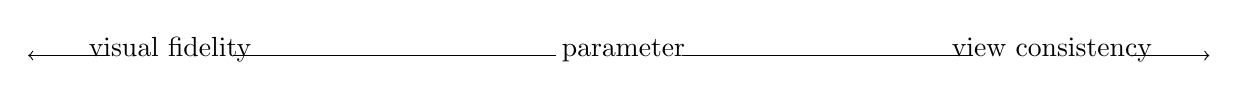
\begin{tikzpicture}
                \draw[<-] (0,0) -- (1,0);
                \draw[-] (2.6,0) -- (6.7,0);
                \draw[-] (8.3,0) -- (12,0);
                \draw[->] (14,0) -- (15,0);
                \node[above] at (1.8,-0.2) {visual fidelity};
                \node[above] at (7.5,-0.2) {$\bias$ parameter};
                \node[above] at (13,-0.2) {view consistency};
            \end{tikzpicture}
        }\\[-4pt]%
        && 0.0 & 0.6 & \textbf{1.2} & \textbf{1.8} & 2.4 & 3.0\\%
        \rotatebox{90}{\hspace*{4em}View 1}&%
        \includegraphics[height=0.14\linewidth, trim=150 0 100 0, clip]{figures/hparams_adjusting/initial_2_overlay.jpg}&%
        \includegraphics[height=0.14\linewidth, trim=200 40 300 460, clip]{figures/hparams_adjusting/0.0_2_overlay.jpg}&%
        \includegraphics[height=0.14\linewidth, trim=200 40 300 460, clip]{figures/hparams_adjusting/0.6_2_overlay.jpg}&%
        \includegraphics[height=0.14\linewidth, trim=200 40 300 460, clip]{figures/hparams_adjusting/1.2_2_overlay.jpg}&%
        \includegraphics[height=0.14\linewidth, trim=200 40 300 460, clip]{figures/hparams_adjusting/1.8_2_overlay.jpg}&%
        \includegraphics[height=0.14\linewidth, trim=200 40 300 460, clip]{figures/hparams_adjusting/2.4_2_overlay.jpg}&%
        \includegraphics[height=0.14\linewidth, trim=200 40 300 460, clip]{figures/hparams_adjusting/3.0_2_overlay.jpg}\\%
        \rotatebox{90}{\hspace*{2em}View 2, $+ 40^\circ$}&
        \includegraphics[height=0.14\linewidth, trim=150 0 100 0, clip]{figures/hparams_adjusting/initial_3_overlay.jpg}&%
        \includegraphics[height=0.14\linewidth, trim=200 40 300 460, clip]{figures/hparams_adjusting/0.0_3_overlay.jpg}&%
        \includegraphics[height=0.14\linewidth, trim=200 40 300 460, clip]{figures/hparams_adjusting/0.6_3_overlay.jpg}&%
        \includegraphics[height=0.14\linewidth, trim=200 40 300 460, clip]{figures/hparams_adjusting/1.2_3_overlay.jpg}&%
        \includegraphics[height=0.14\linewidth, trim=200 40 300 460, clip]{figures/hparams_adjusting/1.8_3_overlay.jpg}&%
        \includegraphics[height=0.14\linewidth, trim=200 40 300 460, clip]{figures/hparams_adjusting/2.4_3_overlay.jpg}&%
        \includegraphics[height=0.14\linewidth, trim=200 40 300 460, clip]{figures/hparams_adjusting/3.0_3_overlay.jpg}\\%
    \end{tabular}%
    \caption{The bias parameter $\bias$ trades between visual fidelity (left insets) and multi-view consistency (right insets). The first column shows the initial asset in two views that condition the diffusion model. The white shapes outline a UV region, which we analyze in the insets to illustrate the impact of the $\bias$ parameter on generated visuals.
    Values between 1.2 and 1.8 strike a good balance in this particular scene.}
    \label{fig:hparams}
\end{figure*}











We evaluate the models at the end of several epochs on the validation set and select the best checkpoint based on the F1 score. The full training hyperparameters are provided in Table \ref{tab6:hparams}. These hyperparameters were chosen based on a hyperparameter search on the validation set. 

\subsection{Evaluation Metrics}

We evaluate the models using the standard F1-score metric for Sequence Labeling tasks (\cite{DBLP:conf/conll/SangM03}). For the text-to-text models, the output of the model is converted into an IOB2 format by splitting the output into words by whitespace. All the models are evaluated using the seqeval library (\cite{seqeval}).

\section{Experiments}
\label{sc6:experiments}

\subsection{Named Entity Recognition}
\label{sc6:ner}

In this section we will present and discuss the experiments in the Named Entity Recognition, Opinion Target Extraction and Event Extraction tasks. 

\begin{table}[htb]
    \centering
    \small
    \adjustbox{max width=\textwidth}{
    \begin{tabular}{@{}lcc|cc|cc|cc|ccc@{}}
    \toprule
     & \multicolumn{2}{c}{mT5-xl} & \multicolumn{2}{c}{mT0-xl} & \multicolumn{2}{c}{\cellcolor[HTML]{FFFFFF}{\color[HTML]{1F1F1F} aya-101}} & \multicolumn{2}{c}{\cellcolor[HTML]{FFFFFF}{\color[HTML]{1F1F1F} Yi-1.5-9B-Chat}} &  &  &  \\
    Lang & Base & Cons. & Base & Cons. & Base & Cons. & Base & Cons. & \multirow{-2}{*}{mDertaV3} & \multirow{-2}{*}{afro-xlmr-large} & \multirow{-2}{*}{GLOT500} \\ \midrule
    English & 93.4 & 93.7 & 93.2 & 93.3 & 93.2 & 93.4 & \cellcolor[HTML]{B7E1CD}94.5 & 94.3 & 93.4 & 93.4 & 92.3 \\ \midrule
    Bambara & 52.5 & 53.4 & 52.8 & 53.8 & 56.0 & \cellcolor[HTML]{B7E1CD}56.2 & 46.0 & 46.7 & 33.8 & 40.0 & 51.1 \\
    Ghomálá & 46.1 & 47.5 & 43.3 & 43.7 & 25.8 & 25.5 & 45.9 & \cellcolor[HTML]{B7E1CD}49.6 & 43.3 & 44.0 & 45.7 \\
    Éwé & 79.8 & 81.0 & 73.4 & 73.6 & 80.1 & \cellcolor[HTML]{B7E1CD}81.2 & 74.4 & 74.8 & 74.4 & 70.3 & 72.1 \\
    Fon & 52.0 & 55.4 & 68.0 & \cellcolor[HTML]{B7E1CD}69.7 & 44.5 & 45.3 & 47.4 & 52.2 & 49.2 & 49.8 & 56.7 \\
    Hausa & 71.3 & 73.8 & 70.0 & 71.9 & 67.9 & 70.1 & 62.0 & 61.3 & 70.7 & \cellcolor[HTML]{B7E1CD}74.1 & 67.2 \\
    Igbo & 72.6 & \cellcolor[HTML]{B7E1CD}77.2 & 55.9 & 61.0 & 53.5 & 54.1 & 55.5 & 57.3 & 58.8 & 72.5 & 62.1 \\
    Kinyarwanda & 71.9 & 73.1 & 71.9 & \cellcolor[HTML]{B7E1CD}74.3 & 67.3 & 69.2 & 48.7 & 53.3 & 65.7 & 67.9 & 66.1 \\
    Luganda & 81.9 & 82.3 & 79.0 & 79.5 & 82.8 & \cellcolor[HTML]{B7E1CD}83.1 & 66.9 & 73.6 & 73.0 & 77.9 & 79.2 \\
    Mossi & 52.5 & 53.7 & 55.4 & 55.7 & 56.7 & 56.7 & 54.4 & \cellcolor[HTML]{B7E1CD}57.1 & 44.6 & 45.7 & 51.4 \\
    Naija & 76.3 & \cellcolor[HTML]{B7E1CD}83.5 & 73.5 & 80.1 & 69.3 & 72.1 & 60.5 & 63.5 & 78.7 & 80.4 & 71.1 \\
    Chichewa & 77.7 & 78.8 & 76.5 & 76.7 & 79.9 & 80.2 & \cellcolor[HTML]{B7E1CD}80.5 & 80.4 & 73.7 & 79.6 & 76.6 \\
    chiShona & 35.2 & 48.2 & 24.3 & \cellcolor[HTML]{B7E1CD}54.0 & 35.2 & 42.8 & 25.8 & 43.0 & 35.8 & 35.2 & 39.8 \\
    Kiswahili & 86.4 & \cellcolor[HTML]{B7E1CD}89.6 & 85.7 & 88.0 & 83.3 & 84.7 & 73.1 & 71.4 & 86.7 & 88.2 & 84.0 \\
    Setswana & 81.0 & 81.3 & 72.3 & 73.5 & 82.1 & \cellcolor[HTML]{B7E1CD}82.6 & 60.4 & 64.0 & 63.1 & 73.3 & 66.8 \\
    Akan/Twi & 60.2 & 61.4 & 60.1 & 61.5 & 64.0 & \cellcolor[HTML]{B7E1CD}64.6 & 49.7 & 55.5 & 49.9 & 40.3 & 55.9 \\
    Wolof & 53.3 & 54.3 & 56.4 & 56.8 & 61.3 & \cellcolor[HTML]{B7E1CD}62.3 & 57.1 & 60.9 & 42.0 & 51.3 & 61.6 \\
    isiXhosa & 30.5 & 40.3 & 27.0 & \cellcolor[HTML]{B7E1CD}55.8 & 34.0 & 40.8 & 22.7 & 32.1 & 24.9 & 26.0 & 26.5 \\
    Yorùbá & 55.1 & \cellcolor[HTML]{B7E1CD}58.5 & 51.0 & 51.3 & 26.0 & 25.8 & 48.9 & 55.4 & 34.1 & 52.5 & 54.4 \\
    isiZulu & 49.4 & 54.9 & 39.2 & \cellcolor[HTML]{B7E1CD}66.7 & 40.5 & 45.0 & 23.5 & 33.7 & 44.7 & 47.1 & 43.3 \\ \midrule
    \textbf{Average MasakhaNER} & 62.4 & \cellcolor[HTML]{B7E1CD}65.7 & 59.8 & 65.7 & 58.4 & 60.1 & 52.8 & 57.1 & 55.1 & 58.7 & 59.6 \\ \bottomrule
    \end{tabular}
    }
    \caption{F1 scores in the Named Entity Recognition Task. Model are trained in English and evaluated in a set of African languages.}
    \label{tab6:NER}
    \end{table}

Table \ref{tab6:NER} presents the performance of our method compared to the baselines in the NER task. All models show comparable performance in English. However, when assessing zero-shot cross-lingual transfer, significant performance differences emerge.

In the zero-shot cross-lingual transfer setting, constrained decoding consistently outperforms unconstrained decoding. For some languages, such as Bambara, Ghomálá, and Éwé, both methods yield similar results. In contrast, other languages, including Shona, isiXhosa, and Zulu, exhibit marked performance improvements. These Southern Bantu languages have unique linguistic features: they capitalize proper names following the noun class prefix (e.g., kweZambia) and display highly inflected morphology (\cite{adelani-etal-2022-masakhaner}). These attributes challenge the cross-lingual transfer abilities of English fine-tuned NER models. Consequently, all baseline models, including the encoder-only variants, perform suboptimally in these languages and are clearly outperformed by our constrained decoding approach.


As demonstrated in Section \ref{sc6:ablation}, text-to-text models struggle with agglutinative languages, frequently mislabeling entities by arbitrarily splitting them into sub-words. Our constrained decoding corrects this by ensuring that the output sentence retains the original words from the input sentence. Overall, constrained decoding excels in the zero-shot cross-lingual setting for languages with highly inflected agglutinative morphology. Although the performance gap is less pronounced for language isolates like Bambara, Éwé, Fon, and Twi, it remains significant.


\begin{table}[htb]
    \centering
    \begin{tabular}{@{}lccc@{}}
    \toprule
    \multicolumn{1}{l}{Model} & Unconstrained & Constrained & \multicolumn{1}{c@{}}{Delta} \\ \midrule
    mT5-xl & 62.4 & 65.7 & \multicolumn{1}{c@{}}{+3.3} \\
    mT0-xl & 59.8 & 65.7 & \multicolumn{1}{c@{}}{+5.9} \\
    aya-101 & 58.4 & 60.1 & \multicolumn{1}{c@{}}{+1.7} \\
    Qwen2-7B-Instruct & 39.7 & 42.0 & \multicolumn{1}{c@{}}{+2.3} \\
    gemma-1.1-7b-it & 46.8 & 49.0 & \multicolumn{1}{c@{}}{+2.2} \\
    Llama-3-8B-Instruct & 51.2 & 52.7 & \multicolumn{1}{c@{}}{+1.6} \\
    aya-23-8B & 51.6 & 52.6 & \multicolumn{1}{c@{}}{+0.9} \\
    Yi-1.5-9B-Chat & 52.8 & 57.1 & \multicolumn{1}{c@{}}{+4.3} \\ \midrule
    GLOT500 & \multicolumn{2}{c}{59.6} & \\
    mDeBERTa-v3 & \multicolumn{2}{c}{55.1} & \\
    Davlan/afro-xlmr-large & \multicolumn{2}{c}{58.7} & \\ \bottomrule
    \end{tabular}
    \caption{Average F1 scores in the MasakhaNER dataset.}
    \label{tab6:ner_mini}
    \end{table}
    



Models exhibit varying performance across languages. For instance, aya-101 achieves the best performance for Éwé, Luganda, Setswana, Twi, and Wolof, while mT0 is superior for languages such as Fon, Kinyarwanda, chiShona, isiXhosa, and Zulu. We attribute this to the different training data used by the models. Nonetheless, we observe that mT5-xl and mT0-xl, combined with our constrained decoding algorithm, outperform encoder-only models by more than 5 points in F1 score on average. This represents a significant improvement over the previous state-of-the-art for zero-shot cross-lingual transfer in NER tasks.



In Table \ref{tab6:ner_mini} we present the average performance of different models on the MasakhaNER dataset. Qwen2, Gemma, and Aya-23 achieve suboptimal results compared to the other text-to-text models. This is likely due to these models being trained on a smaller number of high-resource languages, rendering them less proficient in African languages. However, the results demonstrate that constrained decoding is effective in improving the performance of all text-to-text models in zero-shot cross-lingual transfer.

\subsection{Opinion Target Extraction}
\label{sc6:ote}

\begin{table}[htb]
    \small
    \centering
    \adjustbox{max width=\linewidth}{%
    \begin{tabular}{@{}lcc|cc@{}}
    \toprule
     & \multicolumn{2}{c}{mT0-xl} &  &  \\
    Lang & Base & Cons & \multirow{-2}{*}{\begin{tabular}[c]{@{}c@{}}GLOT\\ 500\end{tabular}} & \multirow{-2}{*}{\begin{tabular}[c]{@{}c@{}}mDeBERTa\\ V3\end{tabular}} \\ \midrule
    English & 82.6 & \cellcolor[HTML]{B7E1CD}{84.8} & 82.6 & 83.6 \\ \midrule
    Spanish & 77.8 & \cellcolor[HTML]{B7E1CD}{79.4} & 69.4 & 78.0 \\
    French & 74.1 & 76.6 & 65.8 & \cellcolor[HTML]{B7E1CD}{76.9} \\
    Dutch & 74.1 & 77.1 & 66.5 & \cellcolor[HTML]{B7E1CD}{77.3} \\
    Russian & 71.1 & 75.7 & 69.2 & \cellcolor[HTML]{B7E1CD}{76.5} \\
    Turkish & 56.8 & \cellcolor[HTML]{B7E1CD}{57.7} & 50.4 & 56.4 \\ \midrule
    Average & 70.8 & \cellcolor[HTML]{B7E1CD}{73.3} & 64.3 & 73.0 \\ \bottomrule
    \end{tabular}
    }
    \caption{F1 scores in the Opinion Target Extraction Task.}
    \label{tab6:OTE}
    \end{table}

In the NER task, we experimented with cross-lingual transfer approaches using a set of low-resource African languages that significantly differ from English. For the Opinion Target Extraction task, we evaluated cross-lingual transfer performance into languages from the Indo-European language family. Due to the high computational cost of the text-to-text models, we only evaluated the best model from the previous task, mT0-XL.

As shown in Table \ref{tab6:OTE}, excluding Turkish (an agglutinative language), the performance decline in the target languages compared to English is less pronounced, suggesting a more seamless transfer. Even in this context, our constrained generation algorithm significantly surpasses the unconstrained generation. Finally, while mT0-XL and mDeBERTa-v3 show comparable performance, our approach demonstrates slightly higher average performance across the board.


\subsection{Event Extraction}
\label{sc6:ee}

\begin{table}[htb]
    \centering
    \small
    \adjustbox{max width=\linewidth}{%
    \begin{tabular}{@{}lcc|cc@{}}
    \toprule
     & \multicolumn{2}{c}{mT0-xl} &  &  \\
    Lang & Base & Cons & \multirow{-2}{*}{\begin{tabular}[c]{@{}c@{}}GLOT\\ 500\end{tabular}} & \multirow{-2}{*}{\begin{tabular}[c]{@{}c@{}}mDeBERTa\\ V3\end{tabular}} \\ \midrule
    English\textsubscript{Entity} & \cellcolor[HTML]{B7E1CD}{95.5} & \cellcolor[HTML]{B7E1CD}{95.5} & 94.5 & 95.3 \\
    Chinese\textsubscript{Entity} & 70.1 & \cellcolor[HTML]{B7E1CD}{73.3} & 34.1 & 54.2 \\ \midrule
    English\textsubscript{Trigger} & \cellcolor[HTML]{B7E1CD}{78.9} & \cellcolor[HTML]{B7E1CD}{78.9} & 74.1 & 78.0 \\
    Chinese\textsubscript{Trigger} & 49.6 & \cellcolor[HTML]{B7E1CD}{52.1} & 0.0 & 30.5 \\ \bottomrule
    \end{tabular}
    }
    \caption{F1 scores in the Event Extraction Task.}
    \label{tab6:EE}
    \end{table}

For the Event Extraction task we aim to perform zero-shot cross-lingual transfer from English to Chinese. This task is particularly challenging due to the vast linguistic and cultural differences between the two languages, including script type, syntax, semantics, and the use of tones in Chinese. As reported in Table \ref{tab6:EE}, both GLOT500 and mDEBERTa struggle with the transfer from English to Chinese, whereas mT0-XL achieves much better results. Consistent with previous evaluations, our constrained generation approach improves over the unconstrained generation method by approximately 3 points in F1 score.

\subsection{Model Transfer vs Data Transfer}
\label{sc6:transfer}

In this chapter we focus on improving the zero-shot model-transfer approach. However, constrained decoding can also be used in conjunction with data transfer. In this section we compare the performance of the constrained decoding algorithm when used in both zero-shot model-based transfer and data transfer settings using the MasakhaNER NER dataset. To this end, we use the automatically generated NER datasets for eight African languages from Chapter \ref{ch:data-transfer}. These datasets were generated by translating the CoNLL2003 (\cite{DBLP:conf/conll/SangM03}) English dataset into the target languages using NLLB200 (\cite{DBLP:journals/corr/abs-2207-04672}) and then projecting the labels using T-Projection. Using the same settings as for the zero-shot approach, we evaluate the performance of the constrained decoding algorithm when fine-tuning the models on the generated datasets. The results are presented in Table \ref{tab6:modelvsdata}. ``Zero'' refers to the models trained with English CoNLL 2003 data and evaluated in the target languages, while "Data" refers to the models fine-tuned on the translated CoNLL 2003 datasets. Both settings use the constrained decoding algorithm.

\begin{table}[htb]
    \centering
    \small
    \adjustbox{max width=\textwidth}{
        \begin{tabular}{@{}l|cc|cc|cc|cc|cc|cc@{}}
            \toprule
            \multicolumn{1}{l}{} & \multicolumn{2}{c}{mDebertaV3} & \multicolumn{2}{c}{mT5-xl}                   & \multicolumn{2}{c}{mT0-xl}               & \multicolumn{2}{c}{aya-101}              & \multicolumn{2}{c}{Llama-3-8B-Instruct} & \multicolumn{2}{c}{Yi-1.5-9B-Chat} \\
            Lang                 & Zero    & Data   & Zero                    & Data & Zero & Data                & Zero & Data                & Zero           & Data          & Zero      & Data     \\ \midrule
            Hausa                & 70.7         & 72.7            & \cellcolor[HTML]{B7E1CD}73.8 & 67.8          & 71.9      & 72.4                         & 70.1      & 72.6                         & 63.5                & 70.1                   & 61.3           & 62.4              \\
            Igbo                 & 58.8         & 71.4            & 77.2                         & 69.9          & 61.0      & 72.9                         & 54.1      & \cellcolor[HTML]{B7E1CD}82.7 & 54.7                & 73.7                   & 57.3           & 58.7              \\
            Chichewa             & 73.7         & 77.2            & 78.8                         & 51.6          & 76.7      & 76.8                         & 80.2      & \cellcolor[HTML]{B7E1CD}83.0 & 78.6                & 68.2                   & 80.4           & 52.4              \\
            chiShona             & 35.8         & 74.9            & 48.2                         & 75.0          & 54.0      & 74.1                         & 42.8      & \cellcolor[HTML]{B7E1CD}77.0 & 25.3                & 65.3                   & 43.0           & 46.2              \\
            Kiswahili            & 86.7         & 85.5            & \cellcolor[HTML]{B7E1CD}89.6 & 77.4          & 88.0      & 85.1                         & 84.7      & 85.4                         & 77.2                & 80.1                   & 71.4           & 65.0              \\
            isiXhosa             & 24.9         & 72.3            & 40.3                         & 53.6          & 55.8      & \cellcolor[HTML]{B7E1CD}74.8 & 40.8      & 74.5                         & 25.8                & 64.8                   & 32.1           & 46.0              \\
            Yorùbá               & 34.1         & 42.7            & 58.5                         & 37.1          & 51.3      & 46.7                         & 25.8      & \cellcolor[HTML]{B7E1CD}60.5 & 34.9                & 56.4                   & 55.4           & 37.6              \\
            isiZulu              & 44.7         & 66.7            & 54.9                         & 64.4          & 66.7      & \cellcolor[HTML]{B7E1CD}71.2 & 45.0      & 64.9                         & 22.5                & 58.0                   & 33.7           & 36.4              \\ \midrule
            Average              & 53.7         & 70.4            & 65.2                         & 62.1          & 65.7      & 71.8                         & 55.5      & \cellcolor[HTML]{B7E1CD}75.1 & 47.8                & 67.1                   & 54.3           & 50.6              \\ \bottomrule
            \end{tabular}
    }
    \caption{F1 Scores for Named Entity Recognition Task. ``Zero'' refers to the model trained in English and evaluated on a set of African languages. ``Data'' refers to the model trained on automatically translated and projected data using T-Projection for each language.}
    \label{tab6:modelvsdata}
    \end{table}

The results show that the zero-shot cross-lingual transfer performance when using text-to-text models such as mT5-xl or mT0-xl is significantly better than the zero-shot performance of mDeBERTa-v3, as we already demonstrated in Section \ref{sc6:ner}. However, mDeBERTa-v3 shows very competitive results in the data-transfer setting. For text-to-text models, the performance of the zero-shot and data-transfer approaches varies across languages. In languages where the model is proficient, such as Hausa or Igbo for mT5-xl, the zero-shot approach outperforms the data-transfer approach. However, in languages where the model is less proficient, such as isiXhosa or Zulu, the data-transfer approach is superior. In the case of aya-101 and LLama-3, which we reported to be less proficient in African languages in Section \ref{sc6:ner}, the data-transfer approach results in a significant performance improvement. In fact, aya-101 outperforms all other models in the data-transfer setting. This suggests that the constrained decoding algorithm can be used in conjunction with data-transfer methods to further improve the performance of models in low-resource languages. 

Similar to the insights from Chapter \ref{ch:model-vs-data}, the results suggest that when a model is proficient in both the source and target languages, model-based transfer is superior to data-based transfer. Thanks to the methodology developed in this chapter, we can now successfully leverage the power of text-to-text LLMs in a zero-shot setting to achieve superior zero-shot cross-lingual transfer results. However, when the model is less proficient in the target language, data-based transfer can be a better option. Data transfer also has the advantage of allowing the use of more efficient models. The results demonstrate that while mDeBERTa-v3 is not competitive in the zero-shot setting, it achieves similar results to the best-performing text-to-text models in the data-transfer setting, despite having fewer parameters and requiring less computational resources.

\section{Ablation Study}
\label{sc6:ablation}

In this section we aim to better understand why and in which scenarios constrained decoding performs better than unconstrained decoding. To achieve this, we identify the types of mistakes that unconstrained decoding makes which are subsequently fixed by constrained decoding. These errors can be grouped into three categories: inconsistent HTML markups, word hallucinations, and word splittings.

\begin{figure}[tb]
    \centering
    \includegraphics[width=0.8\linewidth]{Capitulos/6_ModelTransfer/diagramas/Hallucination.pdf}
    \caption{Percentage of hallucinated words compared to the performance delta between unconstrained and unconstrained beam search in MasakhaNER using mT0-XL.}
    \label{fig6:Hallucination}
\end{figure}

\paragraph{Inconsistent HTML markups:} The model occasionally generates HTML markup that cannot be parsed correctly, such as when a tag is opened but never closed. We found that this occurs in less than 1\% of the annotated sentences. Consequently, it has a negligible effect on the overall performance of the model.

\paragraph{Word hallucinations:} The model sometimes includes in the output a word that was not present in the input. This occurs because unconstrained generation often produces output that mixes English and the target language. For instance, given the sentence \textit{``Kaliforni sullã sẽn togse''}, mT0-XL, when using unconstrained decoding, produces \textit{``<Location> California </Location> sullã sẽn togse''}. In this instance, the model has translated \textit{``Kaliforni''} to \textit{``California''}. Furthermore, inadvertent translation is not the only cause of hallucinations in the output. Perhaps due to a limited understanding of the target language, the model often introduces typos (e.g., \textit{``okudlula''} incorrectly becomes \textit{``okudludlule''}). Interestingly, it even mixes African languages. For instance, given a Zulu sentence as input containing the word \textit{``Musawenkosi''} (God Bless You), the model outputs the very similar Chichewa word \textit{``Mumawenkosi''} (You are welcome).

\paragraph{Word Splittings:} They refer to instances where the model either divides a word into multiple subwords or, conversely, combines several words into a single one. This occurs because the model has been trained in English and, when tested on agglutinative languages, it attempts to mimic English morphology by arbitrarily splitting words. For instance, the sequence \textit{``<Location> waseThekwini </Location> <Person> uShauwn Mkhize </Person>''} becomes \textit{``wase <Location> Thekwini </Location> u <Person> Shauwn Mkhize </Person>''}. This behavior is interesting, as lemmatization is a component of many downstream Information Extraction applications. One could argue that this is the desired behavior. However, although accidental lemmatization was performed correctly in this particular example, this is not usually the case. For instance, in Basque (whose results are not reported here for brevity, although the models were tested in this language), as illustrated in Figure \ref{fig6:constrained_unconstrained}, the model incorrectly splits the term \textit{``Realean''} into \textit{``Reale''} and \textit{``an''}. However, \textit{``Reale''} does not represent the correct lemma, which would correspond to \textit{``Reala''}, the name of a football team. Therefore, the model seems to be arbitrarily splitting words to mimic English morphology.

\begin{figure}[tbp]
    \centering
    \includegraphics[width=\linewidth]{Capitulos/6_ModelTransfer/diagramas/Hallucination_Params.pdf}
    \caption{Average percentage of mistakes generared by Unconstrained Beam search in MasakhaNER using mT0 models of different sizes}
    \label{fig6:HallucinationvsParams}
\end{figure}


We calculate the percentage of sentences containing some of these errors for each language in the NER task when using mT0-XL with unconstrained generation. The results are depicted in Figure \ref{fig6:HallucinationvsParams}. Additionally, we compared the overall percentage of sentences containing any error with the performance difference between constrained and unconstrained generation. The larger the delta, the greater the performance improvement with constrained generation.

Figure \ref{fig6:HallucinationvsParams} indicates that word splitting and hallucinations correlate with the performance delta, suggesting that addressing these issues is key to the superiority of the constrained generation algorithm. It also underscores that unconstrained generation produces a substantial proportion of sentences with errors. In cases like chiShona and isiXhosa (discussed in Section \ref{sc6:ner}), this could affect over 50\% of the output sentences. It should be noted that word splitting has a more pronounced effect on the performance delta than hallucinations. This can be attributed to the standard sequence evaluation method used for these tasks. 

To convert the model's output into IOB2 encoding, we derive annotations such as \textit{"B-LOC O O O"} for the example \textit{``<Location> California </Location> sullã sẽn togse''}. This annotation remains accurate even if the model translates the entity into English. However, when the model splits or merges words, the IOB2 labeling is disrupted, rendering the sentence incorrect in the evaluation. Thus, although the evaluation method may gloss over hallucination errors, it is important to note that models generate a significant number of hallucinations when producing unconstrained predictions, potentially impacting the ultimate efficacy and applicability of IE systems.



We also evaluated the total number of mistakes generated by unconstrained beam search in the NER task with mT0 models of varying sizes. As illustrated in Figure \ref{fig6:HallucinationvsParams}, word splitting and inconsistent HTML markups remain consistent across models with different parameter sizes. However, the frequency of hallucinations decreases as the model size increases. This might be because models with more parameters have a more refined representation of individual languages and therefore mix languages less frequently.

\begin{figure}[tbp]
    \centering
    \includegraphics[width=\linewidth]{Capitulos/6_ModelTransfer/diagramas/F1_Score_by_Model_Parameters.pdf}
    \caption{Average F1 score in MasakhaNER compared to the mT0 model size}
    \label{fig6:F1vsParams}
\end{figure}

Additionally, we assess the average F1 score in the NER task for mT0 models ranging from 300 million to 3.7 billion parameters. The results, presented in Figure \ref{fig6:F1vsParams}, show that as the mT0 model's parameter count increases, the F1 score improves, although we observe diminishing returns beyond 1.2 billion parameters. While our experiments utilize the 3.7 billion parameter mT0-XL, constrained generation surpasses both GLOT500 (a 125 million parameter model) and afro-xlmr-large (355 million parameters) when using an mT0 model with only 580 million parameters. This indicates that the superiority of our method over encoder-only models is not solely due to leveraging a larger model. Notably, with constrained generation, the 580 million parameter mT0 model achieves performance comparable to the 1.2 billion parameter model when the latter employs unconstrained generation. Therefore, constrained generation is also considerably more computationally efficient than its unconstrained counterpart.

\begin{figure}[t]
    \centering
    \includegraphics[width=0.8\linewidth]{Capitulos/6_ModelTransfer/diagramas/Beams_F1.pdf}
    \caption{Average F1 score of mT0-XL in a subset of MasakhaNER compared to the number of beams used for decoding.}
    \label{fig6:BeamsF1}
\end{figure}

Finally, we evaluate the performance of mT0-XL using a varying number of beams. We assess the same checkpoint with beam search ranging from 1 to 8 beams. For these experiments, we utilize a subset of MasakhaNER2, which includes the following languages: Bambara, Ghomálá, Éwé, Fon, Hausa, Igbo, Kinyarwanda, Luganda, and Mossi. As illustrated in Figure \ref{fig6:BeamsF1}, increasing the number of beams has a negligible effect on performance. Considering that the computational cost and GPU memory requirements increase linearly with the number of beams, in this scenario, using a single beam (greedy decoding) offers the best performance-to-cost ratio. This is because the model is highly confident in its top prediction during each step of the decoding process, and introducing additional beams does not significantly diversify or improve the generated outputs.

\section{Conclusion}

In this Chapter we introduce a Constrained Beam Search Algorithm that can be seamlessly incorporated into any text-to-text LLM. We demonstrate that, compared to Unconstrained Beam Search, our algorithm significantly improves zero-shot cross-lingual performance across a broad range of IE tasks and languages. Through an extensive ablation study, we show that constrained generation effectively mitigates issues such as word-splitting and language mixing, which lead to typos and unintentional translations, errors commonly observed when applying text-to-text models to these tasks. Our approach allows the text-to-text mT0 language model to outperform encoder-only models, which had previously set the state-of-the-art standard for zero-shot cross-lingual IE. To the best of our knowledge, we present the best zero-shot cross-lingual results up to date. 

The method developed in this chapter enables model-based cross-lingual transfer for sequence labelling tasks with text-to-text models. This is a significant step forward in the field of zero-shot cross-lingual transfer, as it allows for the use of more powerful models that can handle a wide range of tasks. Considering the prevailing focus on text-to-text LLMs in current research, and the infrequent training of new encoder-only models, we believe that this represents significant progress in this research area. 